\documentclass{article}
\usepackage{graphicx}
\usepackage{subfig}

\begin{document}
    \begin{figure}
        \subfloat[Didascalia immagine 1]{
            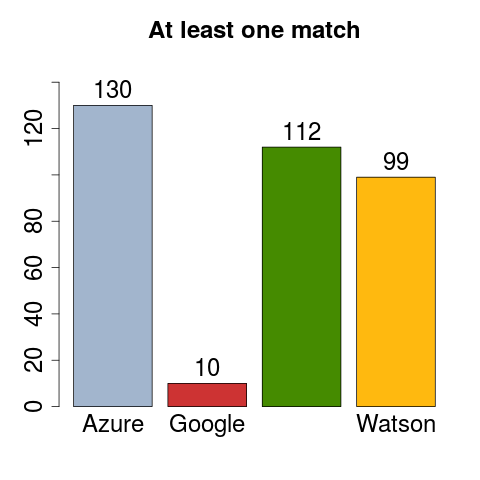
\includegraphics[width=0.45\linewidth]
            {../img/immagine1}
        }
        \hfill
        \subfloat[Didascalia immagine 2]{
            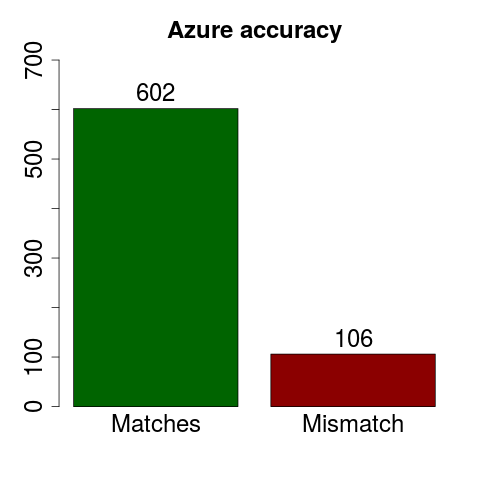
\includegraphics[width=0.45\linewidth]
            {../img/immagine2}
        }
        \\
        \subfloat[Didascalia immagine 3]{
            
\includegraphics[width=\linewidth]
            {../img/immagine3}
        }
        \\
        \subfloat[Didascalia immagine 4]{
            
\includegraphics[width=0.60\linewidth]
            {../img/immagine4}
        }
        \caption{Didascalia globale delle 4 immagini}
    \end{figure}
\end{document}